\pdfminorversion=4
\documentclass[xcolor=table]{beamer}
\usepackage{graphicx}
\usepackage{pdflscape}
\usepackage{float}
\usepackage{multirow}
\usepackage{subfig}
\usepackage{multimedia}

\usetheme{Dresden}

%\setbeamertemplate{itemize body begin}{\tiny}
%\setbeamertemplate{itemize items}[triangle]
%\definecolor{Gray}{gray}{0.85}
%\newcolumntype{header}{>{\columncolor{Gray}}c}
\definecolor{Header}{rgb}{0.2,0.2,0.6}
\definecolor{AlexNet}{gray}{0.60}
\definecolor{Opti}{gray}{0.90}
\definecolor{Even}{gray}{0.90}
\definecolor{Odd}{gray}{0.60}
\definecolor{Imp}{rgb}{0,.85,0}

% Coloring cell with improvement
%\newcommand{\imp}[1]{#1\cellcolor{Imp}}
\newcommand{\imp}[1]{\textbf{#1}}

\newcommand{\tabMultiRow}[4]{%
    \rowcolor{#2}
    & LSTM & %
    #3\\
    \rowcolor{#2}
    \multirow{-2}{*}{#1}%
    & biLSTM &%
    %
    #4
}
%\newcommand{\tabRow}[11]{%
%    \multirow{2}{*}{#1}%
%    & LSTM & %
%    #2\\
%    & #2& #3& #4& #5& #6&\\
%    & biLSTM &%
%    & #7& #8& #9& #10& #11&\\\hline%
%}



\begin{document}

\title{A multi-view Automatic Lip-reading}
\subtitle{Group 12, The Kip-reader's}
\author{Houjeung Han \and Jesper Loenbaek \and Youngsoo Jang}
\institute%
{
    School of Computing\\
    KAIST\\
    Daejeon, Korea
}

\date{5-19 Dec 2016}
\frame{\titlepage}

\begin{frame}{Content}
    \begin{itemize}
        \item About Lip-reading
        \item General approach and challenge
        \item Experimental setup and database
        \item Baseline architecture
        \item Our approach
        \item Result 
        \item Conclusion 
    \end{itemize}
\end{frame}

\begin{frame}{About Lip-reading}
    \begin{itemize}
        \item What is Lip-reading?
        \begin{itemize}
            \item Understanding speech by visually interpreting movement of lips, face and tongue
        \end{itemize}
    \end{itemize}
    \begin{itemize}
        \item Who use it?
        \begin{itemize}
            \item Deaf or head-of-hearing people
            \item People with normal hearing process (McGurk Effect)
        \end{itemize}
    \end{itemize}
\end{frame}

\begin{frame}{Automatic Lip-reading}
    \begin{itemize}
        \item Understand speech from a video stream
        \begin{itemize}
            \item Input: sequence of images
            \item Output: text 
        \end{itemize}
    \end{itemize}
    \begin{center}
    \includegraphics[width=0.8\textwidth]{fig/automaticLipreadingArchi.pdf}   
    \end{center}
\end{frame}

\begin{frame}{Application}
    \begin{itemize}
        \item Enhancing speech recognition
        \begin{itemize}
            \item Combining audio and visual speech recognition 
        \end{itemize}
        \item Visual Password 
        \item Silent speech interface
        \item Forensic video analysis 
    \end{itemize}
\end{frame}

\begin{frame}{General Approach}
    \begin{itemize}
        \item Extract features from individual images
        %\begin{itemize}
        %    \item Different mouth shape
        %\end{itemize}
        \item Correlate features in time
        %\begin{itemize}
        %    \item Difference in visual pronunciation
        %\end{itemize}
        \item Classification 
    \end{itemize}
    \begin{center}
    \includegraphics[width=0.9\textwidth]{fig/alrVisualTempClass.pdf}   
    \end{center}
\end{frame}

\begin{frame}{Challenges}
    \begin{itemize}
        \item Personal dependencies
        \begin{itemize}
            \item Mouth shape 
            \item Visual pronunciation  
        \end{itemize}
    \end{itemize}
    \begin{itemize}
        \item Recording dependencies 
        \begin{itemize}
            \item Change in illumination 
            \item Camera angle
        \end{itemize}
    \end{itemize}
\end{frame}

\begin{frame}{Experimental Setup}
    \begin{itemize}
        \item Speaker dependent
        \begin{itemize}
        \item One person is used for training and testing
        \end{itemize}
        \item Speaker independent
        \begin{itemize}
        \item Different people is used for training and testing
        \end{itemize}
    \end{itemize}
    \begin{itemize}
        \item Single-view 
        \begin{itemize}
        \item Same view used for training and testing
        \end{itemize}
        \item Cross-view 
        \begin{itemize}
        \item One view used for training, other used for testing
        \end{itemize}
        \item Multi-view 
        \begin{itemize}
        \item Multiple-view used for training and testing
        \end{itemize}
    \end{itemize}
    \begin{center}
    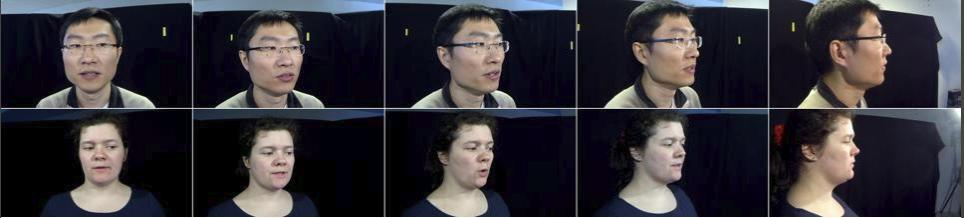
\includegraphics[width=\textwidth]{fig/ouluFullView.jpg}   
    \end{center}
\end{frame}

\begin{frame}{Experimental Setup}
    \begin{itemize}
        \item Speaker dependent
        \begin{itemize}
        \item One person is used for training and testing
        \end{itemize}
        \item \alert{Speaker independent}
        \begin{itemize}
        \item Different people is used for training and testing
        \end{itemize}
    \end{itemize}
    \begin{itemize}
        \item \alert{Single-view}
        \begin{itemize}
        \item Same view used for training and testing
        \end{itemize}
        \item Cross-view
        \begin{itemize}
        \item One view used for training, other used for testing
        \end{itemize}
        \item \alert{Multi-view}
        \begin{itemize}
        \item Multiple-view used for training and testing
        \end{itemize}
    \end{itemize}
    \begin{center}
    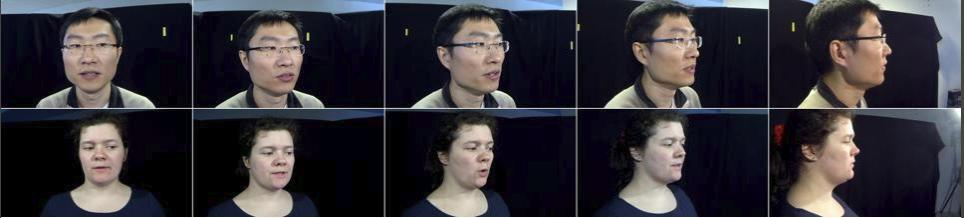
\includegraphics[width=\textwidth]{fig/ouluFullView.jpg}   
    \end{center}
\end{frame}

\begin{frame}{Dataset}
    \begin{columns}[T]
    \column{.65\textwidth}
        \begin{itemize}
            \item Lip-reading challenge (MLAC 2016)%\footnote{http://ouluvs2.cse.oulu.fi/ACCVE.html} (MLAC 2016)
            \item OuluVS2 database
        \end{itemize}
        \begin{itemize}
            \item Recording
            \begin{itemize}
                \item \textbf{52} subjects
                \item \textbf{five} camera angles 
            \end{itemize}
            \item Content 
        \end{itemize}
    \column{.35\textwidth}
        \begin{center}
        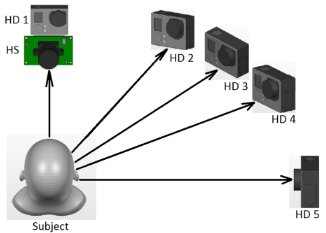
\includegraphics[width=\textwidth]{fig/ouluMultiView.jpg}   
        \end{center}
    \end{columns}
    \begin{center}
    \footnotesize
    \begin{tabular}{l|p{5cm}}
        \multirow{2}{*}{Digits}  
        & "1 7 3 5 1 6 2 6 6 7"\\
        & "4 0 2 9 1 8 5 9 0 4"\\
        \hline
        \multirow{2}{*}{Phrases}  
        & "Thank you"\\
        & "Have a good time"\\
        \hline
        TIMIT & "Chocolate and roses never fail as a romantic gift"
    \end{tabular}
    \end{center}
    %\begin{center}
    %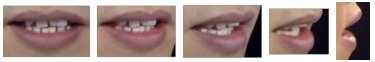
\includegraphics[width=0.8\textwidth]{fig/ouluPreprocessed.jpg}   
    %\end{center}
\end{frame}

\begin{frame}{Baseline}
    \begin{itemize}
        \item State-of-the-art performance (MLAC 2016)
        \item Visual model: Convolutional Neural Network (CNN)
        \item Temporal model: Long Short-Term Memory (LSTM)
        \item Classifier: Support Vector Machine (SVM)
    \end{itemize}
    \begin{center}
    \includegraphics[width=0.8\textwidth]{fig/baseline.pdf}   
    \end{center}
\end{frame}

\begin{frame}{Our Approach}
    \begin{itemize}
        \item Experiment with different architecture
        \begin{itemize}
            \item 1 visual models 
            \item 4 temporal models
            \item 1 Classifier
        \end{itemize}
    \end{itemize}
    \begin{center}
    \includegraphics[width=0.8\textwidth]{fig/ourApproach.pdf}   
    \end{center}
\end{frame}

\begin{frame}{Visual Models}
    \begin{itemize}
        \item CNN
        \begin{figure}
        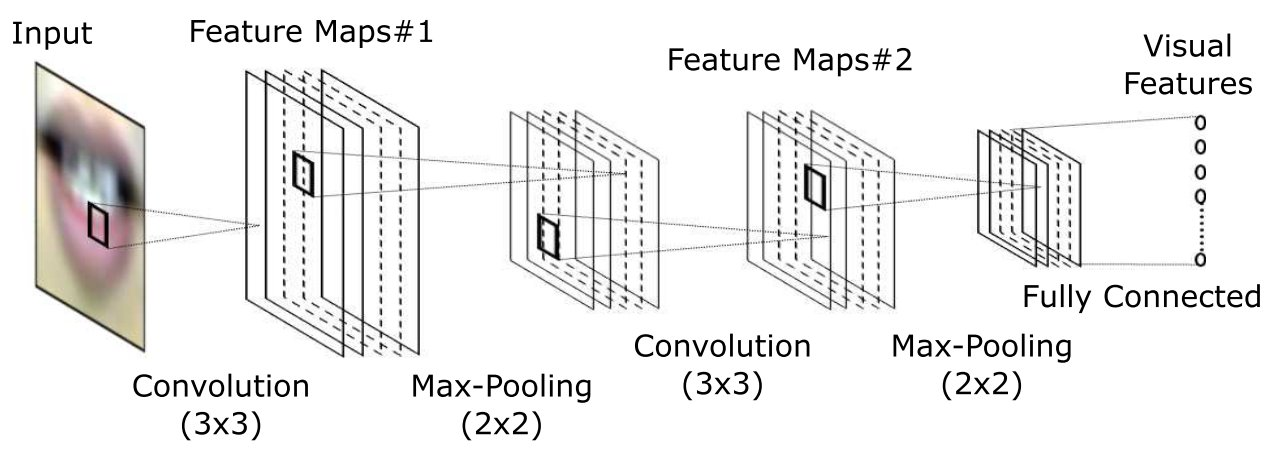
\includegraphics[width=.6\textwidth]{fig/cnnOriginal.jpg}   
        \end{figure}
    \end{itemize}
\end{frame}

%\begin{frame}{Visual Models}
%    \begin{columns}[T]
%    \column{.5\textwidth}
%    \begin{itemize}
%        \item CNN-baseline
%        \begin{figure}
%        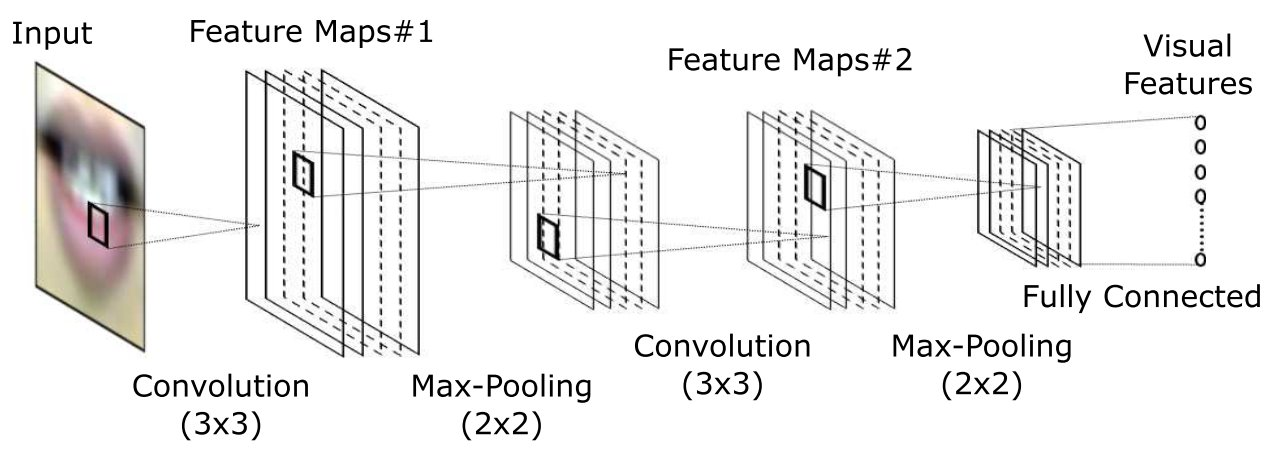
\includegraphics[width=.9\textwidth]{fig/cnnOriginal.jpg}   
%        \end{figure}
%    \end{itemize}
%    \column{.5\textwidth}
%    \begin{itemize}
%        \item 
%        \begin{figure}
%        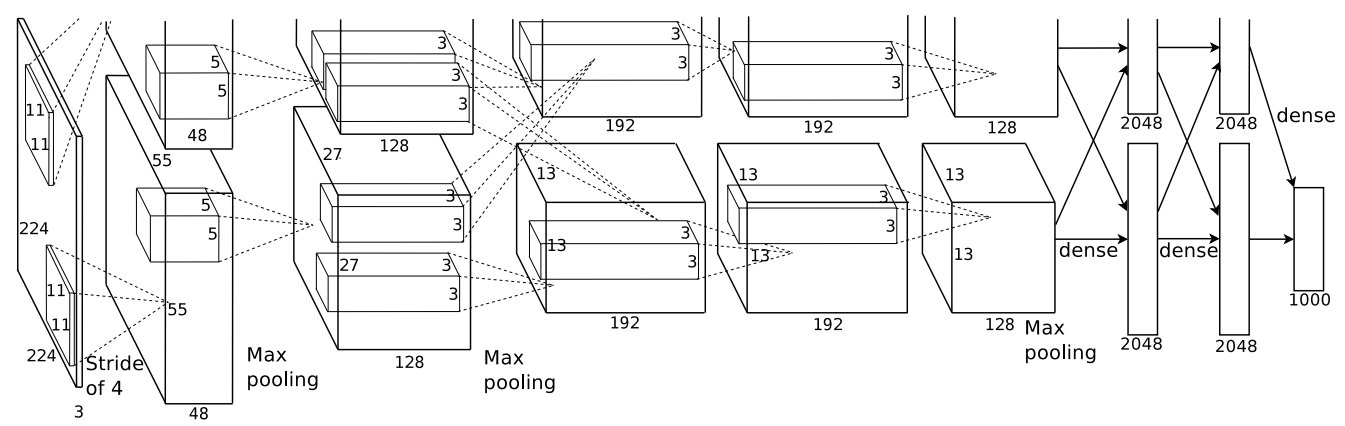
\includegraphics[width=.9\textwidth]{fig/alexNet.jpg}   
%        \end{figure}
%    \end{itemize}
%    \end{columns}
%    %
%    \begin{columns}[T]
%    \column{\textwidth}
%    \begin{itemize}
%        \item Optical Flow 
%        \begin{columns}[T]
%            \column{.25\textwidth}
%            \begin{figure}
%            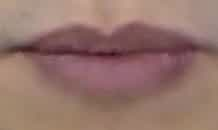
\includegraphics[width=\textwidth]{fig/opti0.jpeg}   
%            \end{figure}
%            \column{.25\textwidth}
%            \begin{figure}
%            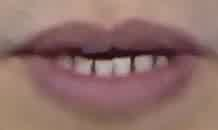
\includegraphics[width=\textwidth]{fig/opti1.jpeg}   
%            \end{figure}
%            \column{.25\textwidth}
%            \begin{figure}
%            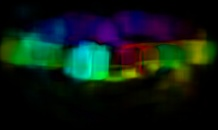
\includegraphics[width=\textwidth]{fig/opti.jpeg}   
%            \end{figure}
%        \end{columns}
%    \end{itemize}
%    \column{.0\textwidth}
%    \end{columns}
%\end{frame}

\begin{frame}{Temporal Models}
    \begin{columns}
    \column{.6\textwidth}
    \begin{itemize}
        \item Long Short-Term Memory (LSTM)
    \end{itemize}
    \vspace{-.5cm}
    \begin{figure}
        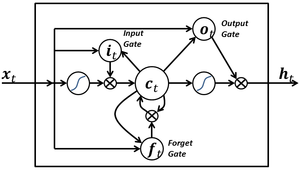
\includegraphics[width=.5\textwidth]{fig/lstm.png}   
    \end{figure}
    \vspace{-.5cm}
    \begin{itemize}
        \item Bidirectional LSTM 
    \end{itemize}
    \vspace{-.5cm}
    \begin{figure}
        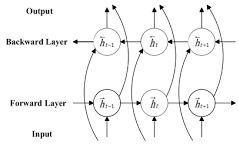
\includegraphics[width=0.5\textwidth]{fig/biLstm.png}   
    \end{figure}
    \column{.4\textwidth}
    \begin{itemize}
        \item Batch-Norm 
    \end{itemize}
    \begin{figure}
        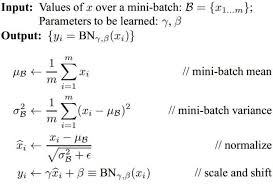
\includegraphics[width=\textwidth]{fig/batchNorm}   
    \end{figure}
    \end{columns}
\end{frame}


\begin{frame}{Architectures}
    \begin{itemize}
        \item 3 new architecture is evaluated
    \end{itemize}
    %
    \begin{center}
    \begin{figure}
        \includegraphics[height=1.3cm]{fig/archiBase.pdf}
    \end{figure}\pause
    \begin{figure}
        \includegraphics[height=1.3cm]{fig/archiBatchNormLstm.pdf}
    \end{figure}\pause
    \begin{figure}
        \includegraphics[height=1.3cm]{fig/archiCnnBiLstm.pdf}
    \end{figure}\vspace{-0.3cm}\pause
    \begin{figure}
        \includegraphics[height=1.3cm]{fig/archiBatchNormBiLstm.pdf}
    \end{figure}
    \end{center}
\end{frame}

\begin{frame}{Results Single-View}
    \vspace{-1.0cm}
    \makebox[\linewidth][r]{%
    \begin{minipage}[t]{0.8\textwidth}
    \begin{figure}
        \begin{overprint}[\textwidth]
            \onslide<1>\hfill\includegraphics[height=1.5cm]{fig/archiBase.pdf}   
            \onslide<2>\hfill\includegraphics[height=1.5cm]{fig/archiBatchNormLstm.pdf}   
            \onslide<3>\hfill\includegraphics[height=1.5cm]{fig/archiCnnBiLstm.pdf}   
            \onslide<4>\hfill\includegraphics[height=1.5cm]{fig/archiBatchNormBiLstm.pdf}   
        \end{overprint}
    \end{figure}
    \vspace{-.1cm}
    \end{minipage}%
    }
    %
    \makebox[\linewidth][c]{%
    \begin{minipage}{1.1\textwidth}
    \begin{center}
    \begin{tabular}{cc|cccccc}
        \rowcolor{Header}
        \multicolumn{2}{c|}{Architecture} &%
        \multicolumn{5}{c}{View} &\\ 
        \rowcolor{Header}
        Visual  & Temporal %
        & 0& 30 & 45 & 60 & 90 & Avg \\\hline\hline
        %
        %
        CNN & LSTM % 
        &81.1 &80.0 &76.9 &69.2 &82.2 &77.9\pause \\\hline
        %
        \rowcolor{Even}
        CNN & LSTM+BN % 
        &80.6 &77.8 & \imp{78.6}& \imp{74.0}& 72.8& 76.7\pause \\\hline
        \rowcolor{Odd}
        CNN & biLSTM % 
        &81.1 &80.0 & \imp{83.9} & \imp{75.8} & \imp{82.5} & \imp{80.7}\pause \\\hline
        \rowcolor{Even}
        CNN & biLSTM+BN % 
        &\imp{84.7} & \imp{81.4} & \imp{82.8} & \imp{77.0} & 81.1& \imp{81.4}\\\hline
    \end{tabular}
    \end{center}
    \end{minipage}%
    }
\end{frame}

\begin{frame}{Architecture Multi-view}
    \begin{itemize}
        \item Dublication of sigle-view visual model
        \item Feature merge before temporal model
    \end{itemize}
    \begin{figure}
        \includegraphics[width=0.8\textwidth]{fig/archiMultiView.pdf}
    \end{figure}
\end{frame}

\begin{frame}{Result Multi-View}
    \begin{center}
    \begin{tabular}{cc|c}
        \rowcolor{Header}
        \multicolumn{2}{c|}{Architecture} &\\
        \rowcolor{Header}
        Visual  & Temporal & Multi-View \\\hline\hline
        %
        %
        CNN & LSTM % 
        & 80.0\\
        \rowcolor{Even}
        CNN & LSTM+BN % 
        & \imp{82.2}\\
        \rowcolor{Odd}
        CNN & biLSTM % 
        & \imp{81.1}\\
        \rowcolor{Even}
        CNN & biLSTM+BN % 
        & \imp{88.1}\\
    \end{tabular}
    \end{center}
\end{frame}

\begin{frame}{Augmenting Data}
    \begin{itemize}
        \item Improving performance by increasing the traning data
        \item Images from camera angles next to each other is similar  
    \end{itemize}\pause
    \begin{figure}
        \includegraphics[width=0.8\textwidth]{fig/augmenting.pdf}
    \end{figure}\pause
    %
    \begin{center}
    \begin{tabular}{cc|cc}
        \rowcolor{Header}
        \multicolumn{2}{c|}{Architecture} &%
        &\\
        \rowcolor{Header}
        Visual  & Temporal %
        & Non-augmented & Augmented\\\hline\hline
        %
        %
        \multicolumn{2}{c|}{Baseline}%
        & 80.0 & \imp{82.1}\\\hline
        %
        \rowcolor{Even}
        CNN& biLSTM % 
        & 81.1 & \imp{81.9}\\\hline
        \rowcolor{Odd}
        CNN& biLSTM+BN % 
        & 88.1 & \imp{88.9}\\\hline
    \end{tabular}
    \end{center}
\end{frame}

%\begin{frame}{Result Augmenting Data}
%\begin{center}
%\begin{tabular}{cc|cc}
%    \rowcolor{Header}
%    \multicolumn{2}{c|}{Architecture} &%
%    &\\
%    \rowcolor{Header}
%    Visual  & Temporal %
%    & Multi& Augmented\\\hline\hline
%    %
%    %
%    \multicolumn{2}{c|}{Baseline}%
%    & 80.0 & 82.1\imp\\\hline
%    %
%    \rowcolor{Even}
%    CNN-base & biLSTM % 
%    & 81.1 & 81.9\imp\\\hline
%\end{tabular}
%\end{center}
%\end{frame}

\begin{frame}{Conclusion}
    \begin{itemize}
        \item 3 different Auto lip-reading architectures is evaluated\pause
        \item 2 experimental setup: \textit{single-view} and \textit{multi-view}\pause
        \item Best performance: CNN combined with a bidirectional-LSTM and batch norm
        \begin{center}
        \begin{tabular}{c|cc}
            \rowcolor{Header}
            Architecture & Single-view Avg & Multi-view\\\hline
            %
            Baseline & 77.9 & 80.0\\
            CNN+biLSTM+BN & \imp{81.4}  & \imp{88.1}\\
        \end{tabular}
        \end{center}\pause
        \item Adjacent views can be used for augmenting training data in multi-view.\pause
        \begin{center}
        \begin{tabular}{c|cc}
            \rowcolor{Header}
            Architecture & Non-augmented & Augmented\\\hline
            %
            Baseline & 80.0 & \imp{82.1}\\
            CNN+biLSTM+BN & 88.1 & \imp{88.9}\\
        \end{tabular}
        \end{center}
    \end{itemize}
\end{frame}

\begin{frame}
\begin{center}
    {\Huge\color[rgb]{0.2,0.2,0.7}%
    Questions?%
    }
\end{center}
\end{frame}

%\bibliographystyle{plain}
% %argument is your BibTeX string definitions and bibliography database(s)
%\bibliography{tmp,mendeley}

\end{document}
